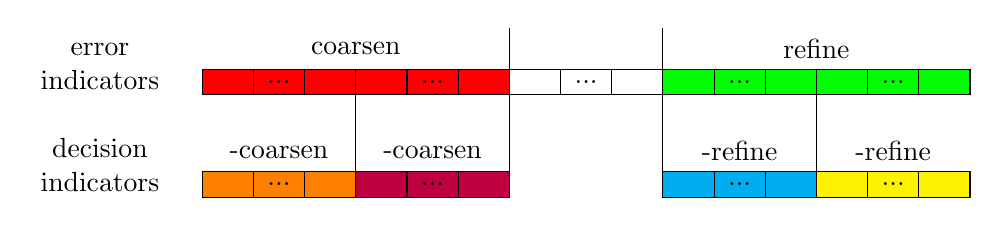
\begin{tikzpicture}[
  scale=0.65,
  valign/.style={%
    text height=1.5ex,
    text depth=.25ex,
  }
]

% error indicators
\node[align=center, text width = 1.6cm] at ( -2,0.55) {error indicators};

\node[align=center] at ( 3,.9) {coarsen};
\fill[color=red] (0,0) rectangle (6,0.5);
\node[align=center] at ( 12,.9) {refine};
\fill[color=green] (9,0) rectangle (15,0.5);

\draw (0,0) rectangle (15,0.5);
\foreach \x in {1,...,14}
  \draw (\x,0) -- (\x,0.5);
\foreach \x in {0,...,4}
  \node[align=center] at (3*\x+1.5,0.25) {...};

\draw (6,1.3) -- (6,-2);
\draw (9,1.3) -- (9,-2);


% decision indicators
\node[align=center, text width = 1.6cm] at ( -2,-1.37) {decision indicators};

% hp coarsen
\node[valign,align=center] at ( 1.5,-1.1) {\p-coarsen};
\fill[color=orange] (0,-2) rectangle (3,-1.5);
\node[valign,align=center] at ( 4.5,-1.1) {\h-coarsen};
\fill[color=purple] (3,-2) rectangle (6,-1.5);

\draw (0,-2) rectangle (6,-1.5);
\foreach \x in {1,...,5}
  \draw (\x,-2) -- (\x,-1.5);
\foreach \x in {0,...,1}
  \node[align=center] at (3*\x+1.5,-1.75) {...};

\draw (3,0) -- (3,-2);

% hp refine
\node[align=center] at (10.5,-1.1) {\h-refine};
\fill[color=cyan] (9,-2) rectangle (12,-1.5);
\node[align=center] at (13.5,-1.1) {\p-refine};
\fill[color=yellow] (12,-2) rectangle (15,-1.5);

\draw (9,-2) rectangle (15,-1.5);
\foreach \x in {10,...,14}
  \draw (\x,-2) -- (\x,-1.5);
\foreach \x in {3,...,4}
  \node[align=center] at (3*\x+1.5,-1.75) {...};

\draw (12,0) -- (12,-2);
\end{tikzpicture}